% !TEX TS-program = pdflatex

\documentclass[unicode,11pt,notheorems,xcolor=table]{beamer}

\usepackage[T2A]{fontenc}
\usepackage[utf8]{inputenc}
\usepackage[russian]{babel}
\usepackage{amsmath,amsfonts,amssymb,amsthm}
\usepackage{mathtools}
\usepackage{diagbox}

\usepackage{ulem}
\usepackage{tikz, graphicx}
%\usepackage{tkz-graph}
\usetikzlibrary{matrix,arrows,decorations.pathmorphing, arrows.meta,positioning}
\usetikzlibrary{positioning,calc}
\usetikzlibrary{petri}
\usetikzlibrary{decorations.pathreplacing}

%Описание стиля презентации
\usetheme[sidebar=0]{kfmn} 
\setbeamercovered{transparent}

%\definecolor{cyan}{RGB}{240,217,1}
%\definecolor{vgugreen}{RGB}{143,188,103}
%\definecolor{vgured}{RGB}{234,38,40}
%\definecolor{vgublue}{RGB}{53,101,167}



\makeatletter
	\g@addto@macro{\endtabular}{\rowfont{}}% Clear row font
	\makeatother
	\newcommand{\rowfonttype}{}% Current row font
	\newcommand{\rowfont}[1]{% Set current row font
		\gdef\rowfonttype{#1}#1\ignorespaces%
	}
\makeatother

\newcommand{\myunit}{9mm}
\tikzset{
    node style sp/.style={draw,circle,minimum size=\myunit},
    node style ge/.style={circle,minimum size=\myunit},
    arrow style mul/.style={draw,sloped,midway,fill=white},
    arrow style plus/.style={midway,sloped,fill=white},
}

%[0, 6, 8, 8, 10, 5, 6, 10, 8, 10, 10], 

\pgfdeclareimage[height=8mm]{university-logo}{logo-iem.png}
\logo{\pgfuseimage{university-logo}}
%2[0, 11, 10, 8, 11, 5, 11, 11, 8, 11, 10, 11],

\titlepicture{
	\begin{tikzpicture}[y=1.4cm,overlay,rotate=8]
	\coordinate (O) at (-3cm,0.9cm);
	\filldraw[thick,draw= vgublue, fill=vgublue!20!white] (0,0) circle[radius=4.2cm];
	\clip (0,0) circle[radius=4.2cm];
	\draw (-1.5,1.5) node{
	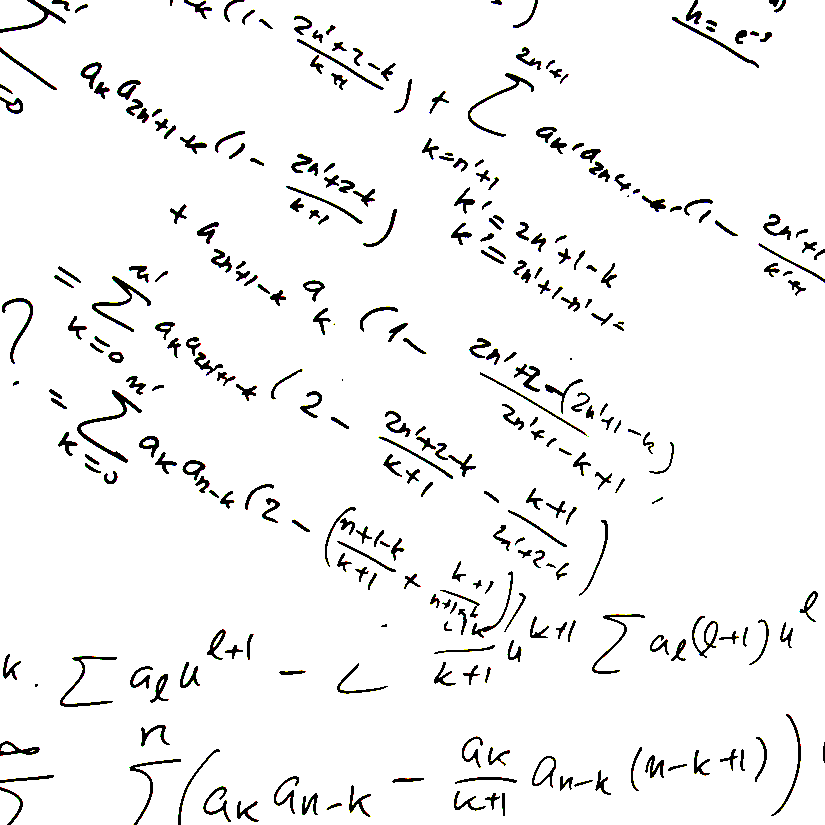
\includegraphics[width=8cm]{titlepic.png}
	};
\end{tikzpicture}
}

\usepackage[math]{iwona}

\newcommand{\hplus}{\mathbin{\hat+}}
\newcommand{\hdot}{\mathbin{\hat\cdot}}
% Описание теорем
\newtheorem{theorem}{Теорема}
\newtheorem{seq}{Следствие}
%%

\LECT % 

% Титульный лист теорем
\author[Д.\,В. Чупраков]{канд.\,физ.-матем.\,наук, доцент Д.\,В. Чупраков\\[6pt] usr10381@vyatsu.ru}

\institute[ВятГУ]{ФГБОУ ВО Вятский государственный университет}

\department{Факультет экономики и финансов}

\title[Лекция~12. Случайные события и вероятности]{
	Введение в экономико-математическое моделирование\\[12pt]
	Лекция~12. Случайные события и вероятности}

\date{25 ноября 2020~г.}


\setbeamercovered{invisible}



\begin{document}


\maketitle

\begin{frame}{Структура лекции}
	\tableofcontents
\end{frame}

\section{Подходы к определению вероятности события}

\subsection{Понятие случайного события и вероятности}

\subsection{Статистическая вероятность}

\begin{frame}{Случайное явление}{}

    \alert{Случайным} называется эксперимент, результат которого нельзя предсказать заранее. 
    
    \medskip
    Невозможность предсказать исход заранее~--- основное, что отличает случайное явление от детерминированного. 

    \medskip
    Методами теории вероятностей можно изучать а лишь те случайные явления $A$, которые:
    \begin{itemize}
        \item могут быть воспроизведены в одних и тех же условиях;
        \item обладают свойством статистической устойчивости: если $A$~--- некоторое событие, могущее произойти или не произойти в результате эксперимента, то~и~доля~$\frac{n(A)}{n}$ числа экспериментов, в которых данное явление произошло, стабилизируется к некоторому числу~$p(A)$. 
    \end{itemize}

\end{frame}    
\begin{frame}{}{}
        Число~\alert{$p(A)$} служит объективной характеристикой возможности появления события~$A$ и называется \alert{вероятностью} явления~$A$.
    
    \medskip
    \begin{block}{Статистическая вероятность}
        Формула
    $$
       \alert{p(A) = \lim_{n \to \infty} \frac{n(A)}{n}},
    $$
    где $n(A)$~--- число появлений события $A$ в $n$ опытах,
    называется \alert{статистическим определением вероятности.}
    \end{block}

    \medskip

    На практике используется приближенная формула
    $$
        \alert{p(A) \approx \frac{n(A)}{n}, \qquad n\text{~--- достаточно большое}}
    $$
\end{frame}

\subsection{Исходы и события}

\begin{frame}{Пространство элементарных исходов}{}
    Понятие пространства элементарных исходов является базовым для теории вероятностей,
    так же как понятие точки в геометрии.
    
    \begin{block}{}
        Под \alert{пространством элементарных исходов $\Omega$} понимается множество, содержащее ее возможные результаты данного случайного эксперимента, из которых в действительности происходит ровно один. 
    \end{block}

    Элементы множества $\omega \in \Omega$, называются \alert{элементарными исходами}.
    
\end{frame}    
\begin{frame}{Примеры пространств элементарных исходов}{}
    Пространство элементарных исходов является 
    \begin{itemize}
        \item \alert{дискретным}, если оно имеет конечное или счетное число элементов;
        \item \alert{непрерывным}, если все точки отрезка, концами которого являются исходы так же являются исходами.
    \end{itemize}

    \medskip
    \structure{Примеры:}
    \begin{itemize}
        \item При броске игральной кости $\Omega=\{1,2,3,4,5,6\}$~--- дискретное пространство;
        \item При стрельбе в мишень~--- точка листа с мишенью~--- непрерывное пространство.
    \end{itemize}
\end{frame}
\begin{frame}{Событие}
    В результате эксперимента \alert{произошло событие $A \subseteq \Omega$}, если в~результате эксперимента произошел один из элементарных исходов $\omega \in A$. 
    
    \begin{block}{}
        \begin{itemize}
            \item \alert{Событием} называется любое множество $A$ пространства исходов $\Omega$.
            \item \alert{Благоприятным исходом события $A$} называется любой исход $\omega \in A$.
        \end{itemize}
    \end{block}
\end{frame}
\begin{frame}{Виды событий}
    \begin{itemize}
        \item \alert{Достоверное событие $\Omega$}~--- событие, содержащее все исходы пространства  $\Omega$. Достоверное событие всегда происходит в~опыте $\Omega$.
        \item \alert{Невозможное событие $\varnothing$}~--- событие, содержащее пустое множество исходов пространства $\Omega$. Невозможное  событие никогда не происходит в опыте $\Omega$.
        \item \alert{Противоположное событие $\bar{A}$}~--- состоит из всех исходов, не~благоприятных для $A$. Оно происходит тогда и только тогда, когда не наступает $A$
        \item \alert{Сумма событий $A+B$}~--- событие, состоящее из всех исходов, содержащихся в событии $A$ или в $B$. Наступает, если наступит $A$ или $B$.
        \item \alert{Произведение $AB$}~--- событие, состоящее из всех исходов благоприятных как для $A$, так и для $B$. Наступает, лишь тогда, когда наступят $A$ и $B$ вместе.
    \end{itemize}

 \end{frame}

 \subsection{Классическая вероятность}
\begin{frame}{Определение вероятности}{}
    Рассмотрим дискретное пространство  элементарных исходов
    $$
        \Omega = \{\omega_1, \omega_2, \ldots, \omega_n \}
    $$

    Каждому элементарному исходу $\omega_i$ сопоставим число~$p_i$ так, что 
        $$
            p_1+p_2+\ldots+p_n = 1
        $$
        
        Назовем $p_i$~--- \alert{вероятностью исхода $\omega_i$.}

    \begin{block}{Определение}
        \alert{Вероятностью события $A\subseteq \Omega$} называется величина, равная сумме вероятностей исходов, благоприятных для события $A$:
        $$
            p(A) = \sum_{\omega\in A} p(\omega)
        $$
        
    \end{block}
\end{frame}

\begin{frame}{Определение классической вероятности}{}
    \begin{block}{Классическая вероятность}
    Если 
    \begin{enumerate}
        \item число исходов $n$ \underline{конечно},
        \item все исходы \underline{равновозможны}: $p(\omega)=\frac{1}{n}$  для каждого $\omega \in \Omega$,
    \end{enumerate}
    то вероятность каждого события $A$ может быть найдена по формуле
    $$
        \alert{P(A) = \frac{n_A}{n}}
    $$
    где $n_A$~---количество исходов, благоприятных событию~$A$.
\end{block}

Приведенная формула носит название классической вероятности и\\ \alert{\Large применима только при указанных условиях!}
\end{frame}

\subsection{Воспоминание о комбинаторике}
\begin{frame}{Комбинаторные принципы}{}
    Формула классической вероятности сводит задачу к вычислению количества элементов множества, то есть делает ее \underline{комбинаторной}.

    \begin{block}{Комбинаторный принцип умножения}
        Если элемент \alert{$A$} можно выбрать \alert{$n$} способами, и при \underline{любом выборе~\alert{$A$}} элемент \alert{$B$} можно выбрать \alert{$m$} способами, то \underline{упорядоченную} пару \alert{$(A, B)$} можно выбрать \alert{$n\cdot m$} способами.
    \end{block}

    \begin{block}{Комбинаторный принцип сложения}
        Если элементы \alert{$A$} и \alert{$B$} нельзя выбрать одновременно, при этом существует \alert{$n$} способов выбрать элемент \alert{$A$} и \alert{$m$}способов выбрать \alert{$B$}, то выбрать \alert{$A$ или $B$} можно \alert{$n + m$} способами. 
    \end{block}

    \begin{itemize}
        \item Принцип умножения позволяет решать задачу поэтапно,
        \item принцип сложения~--- разбивать ее на частные случаи.
    \end{itemize}
\end{frame}

\begin{frame}{Примеры решения задач}
    
\end{frame}

\begin{frame}{Комбинаторные соединения}
    Комбинаторная задача очень часто сводится к подсчету конструкций элементов некоторого множества.
    
    \medskip
    Типичными конструкциями являются:
    \begin{itemize}
        \item \alert{Кортежи}~--- конечные последовательности $(a_1, a_2, \ldots a_n)$ в которых важен порядок следования элементов.
        \item \alert{Наборы}~--- конечные конструкции $\{a_1, a_2, \ldots a_n\}$ в которых порядок следования элементов не важен, но элементы могут повторяться.
    \end{itemize}
    
    \medskip
    Такие конструкции будем называть \alert{комбинаторными соединениями.}
\end{frame}

\begin{frame}{Свойства комбинаторных соединений}
    \structure{Свойства:}
    \begin{itemize}
        \item Упорядоченность~--- важен ли порядок следования элементов.
        \item Состав соединения~--- важно ли какие элементы входят в соединение.
        \item Повторяемость элементов~--- могут ли в соединение входить одинаковые элементы.
    \end{itemize}
    
\end{frame}

\begin{frame}{Перестановки без повторений} 

    \begin{block}{Определение}
        Рассмотрим множество $A$, состоящее из $n$ элементов.
        \alert{Перестановкой} называется кортеж, состоящий из всех элементов  множества $A$, взятых по одному разу.
    \end{block}
    $$
        \alert{P_n = n!}
    $$

    Перестановки различаются только порядком элементов!

    \bigskip
    {\centering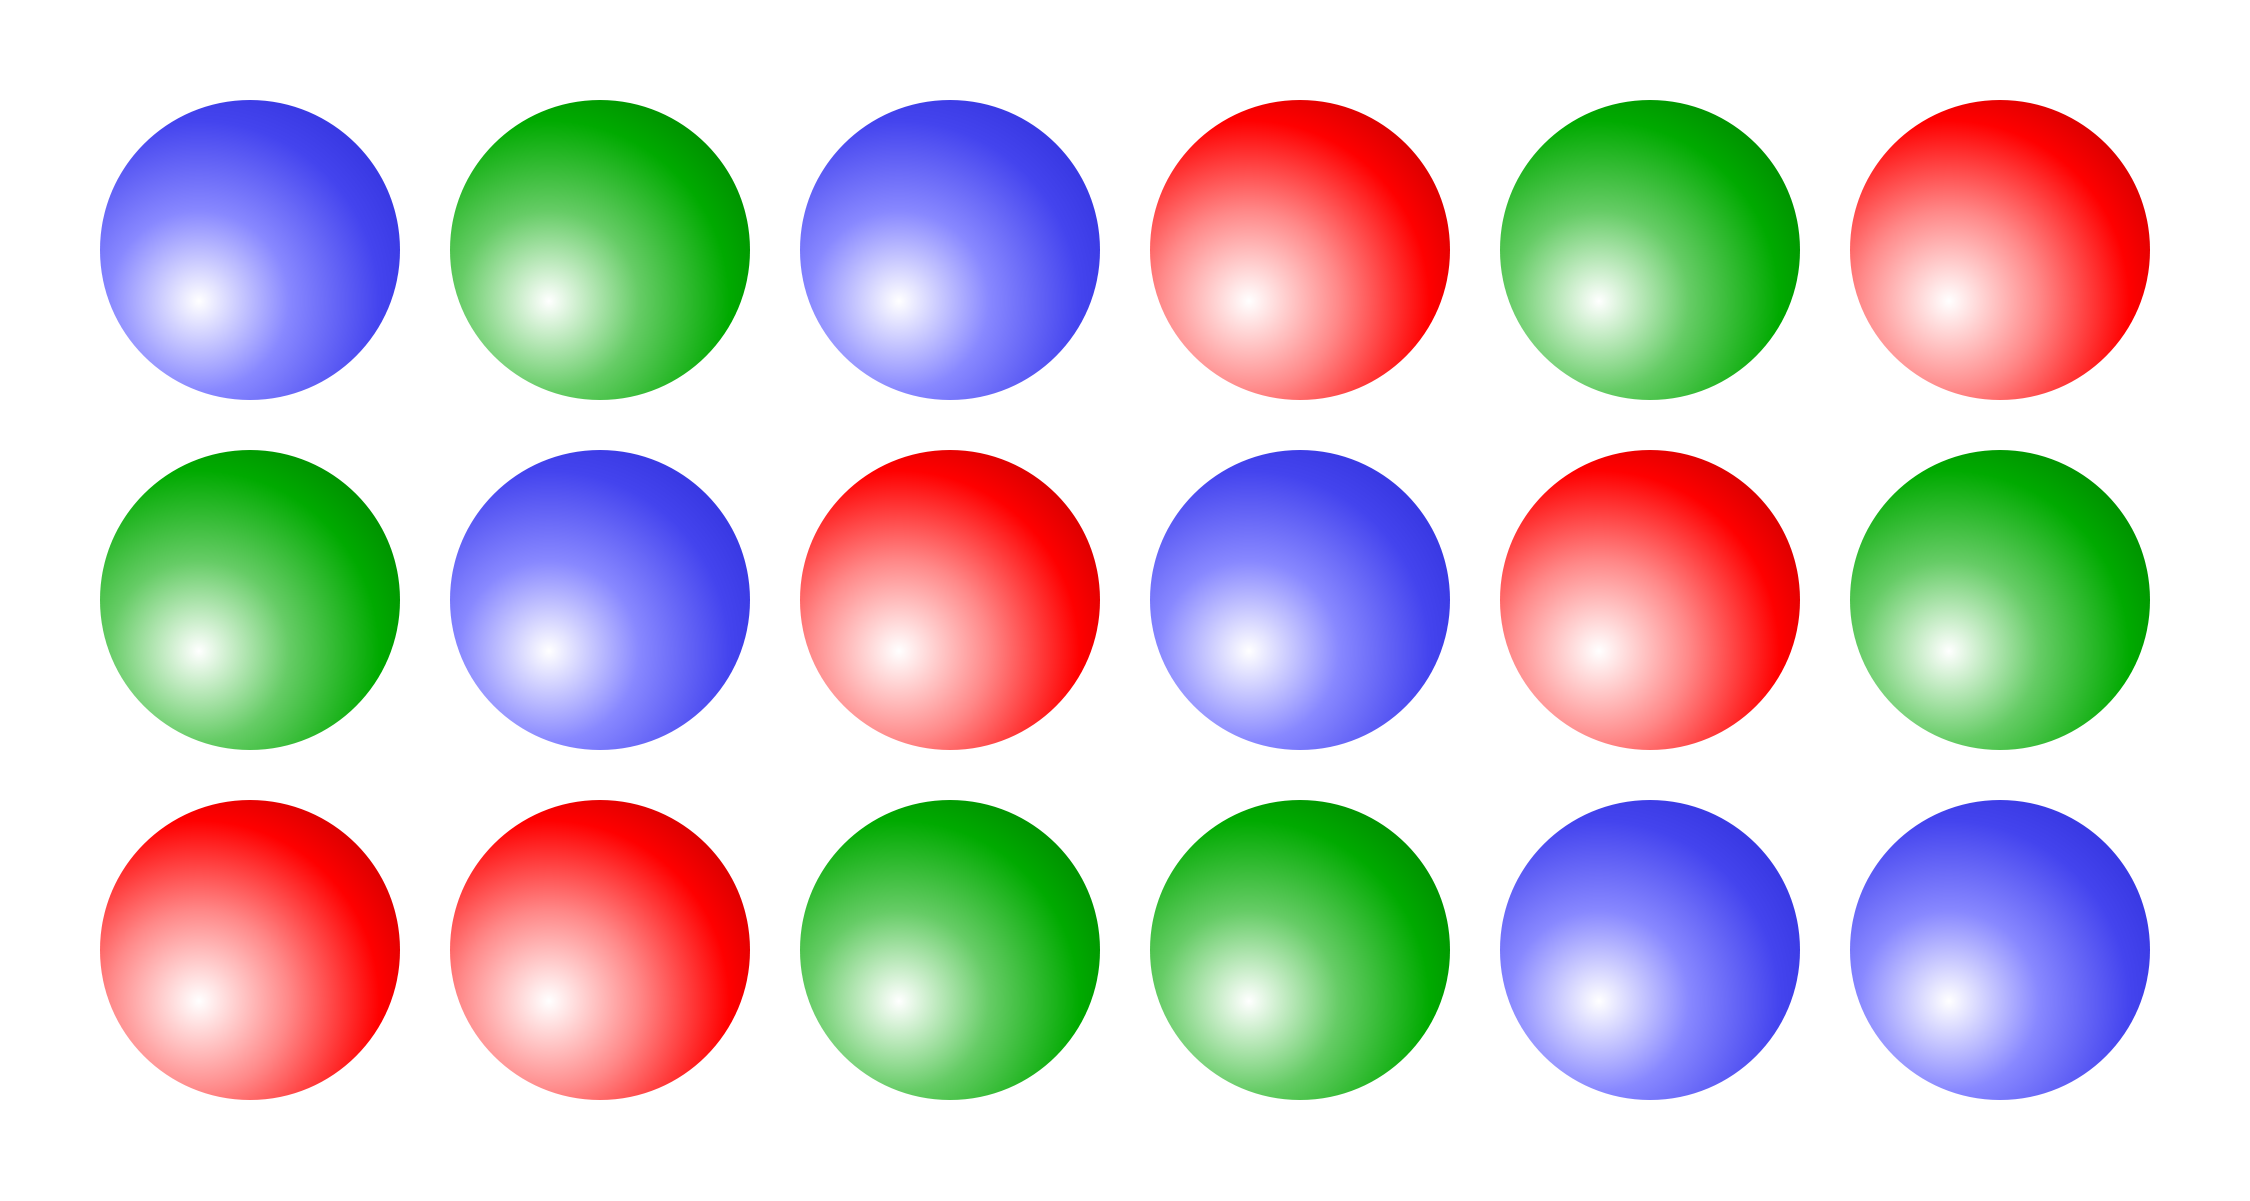
\includegraphics[width=0.4\textwidth]{permutations.png}\par}

\end{frame}
\begin{frame}{Пример. Перестановки без повторений}
    \begin{exampleblock}{}
        Восемь различных книг расставлены наудачу на одной книжной полке. Найти вероятность того, что две определенные книги окажутся поставленными рядом.    
    \end{exampleblock}
    \begin{itemize}
        \item Так как число книг конечно и расстановки произвольны можно пользоваться формулой классической вероятности. 
        
        \item Количество исходов: Расставляются все книги. Важен порядок. Книги на полке не повторяются. Это сочетания без повторений:
        $n=P_8=8!$
        \item Событие $A$~--- две определенные книги 1 и 2 стоят рядом .
        \item 
        Число благоприятных исходов $n(A)$: Склеим книги \texttt{1} и \texttt{2} в \texttt{12}. Расставить 7 книг можно $n_1=P_7=7!$ способами.  
        \item Склеим книги \texttt{1} и \texttt{2} в \texttt{21}. Расставить полученные 7 книг можно $n_1=P_7=7!$ способами.  
        \item Итак,  $n(A)=n_1+n_2=2\cdot 7!$, \hfill \alert{$p(A)=\frac{2\cdot 7!}{8!}=0.25$.}
    \end{itemize}
\end{frame}

\begin{frame}{Перестановки с повторениями} 
        \begin{block}{Определение}
        Пусть каждый  элемент $a_i\in A$ входит в кортеж ровно $k_i$ раз. Такой кортеж называется \alert{перестановкой с повторениями}.
    \end{block}
    $$
        \alert{\tilde{P}(k_1,k_2,\ldots, k_n) = \frac{(k_1+k_2+\ldots+ k_n)!}{k_1!\cdot k_2!\cdot \ldots \cdot k_n!}
        }
    $$
    
    \bigskip
    {\centering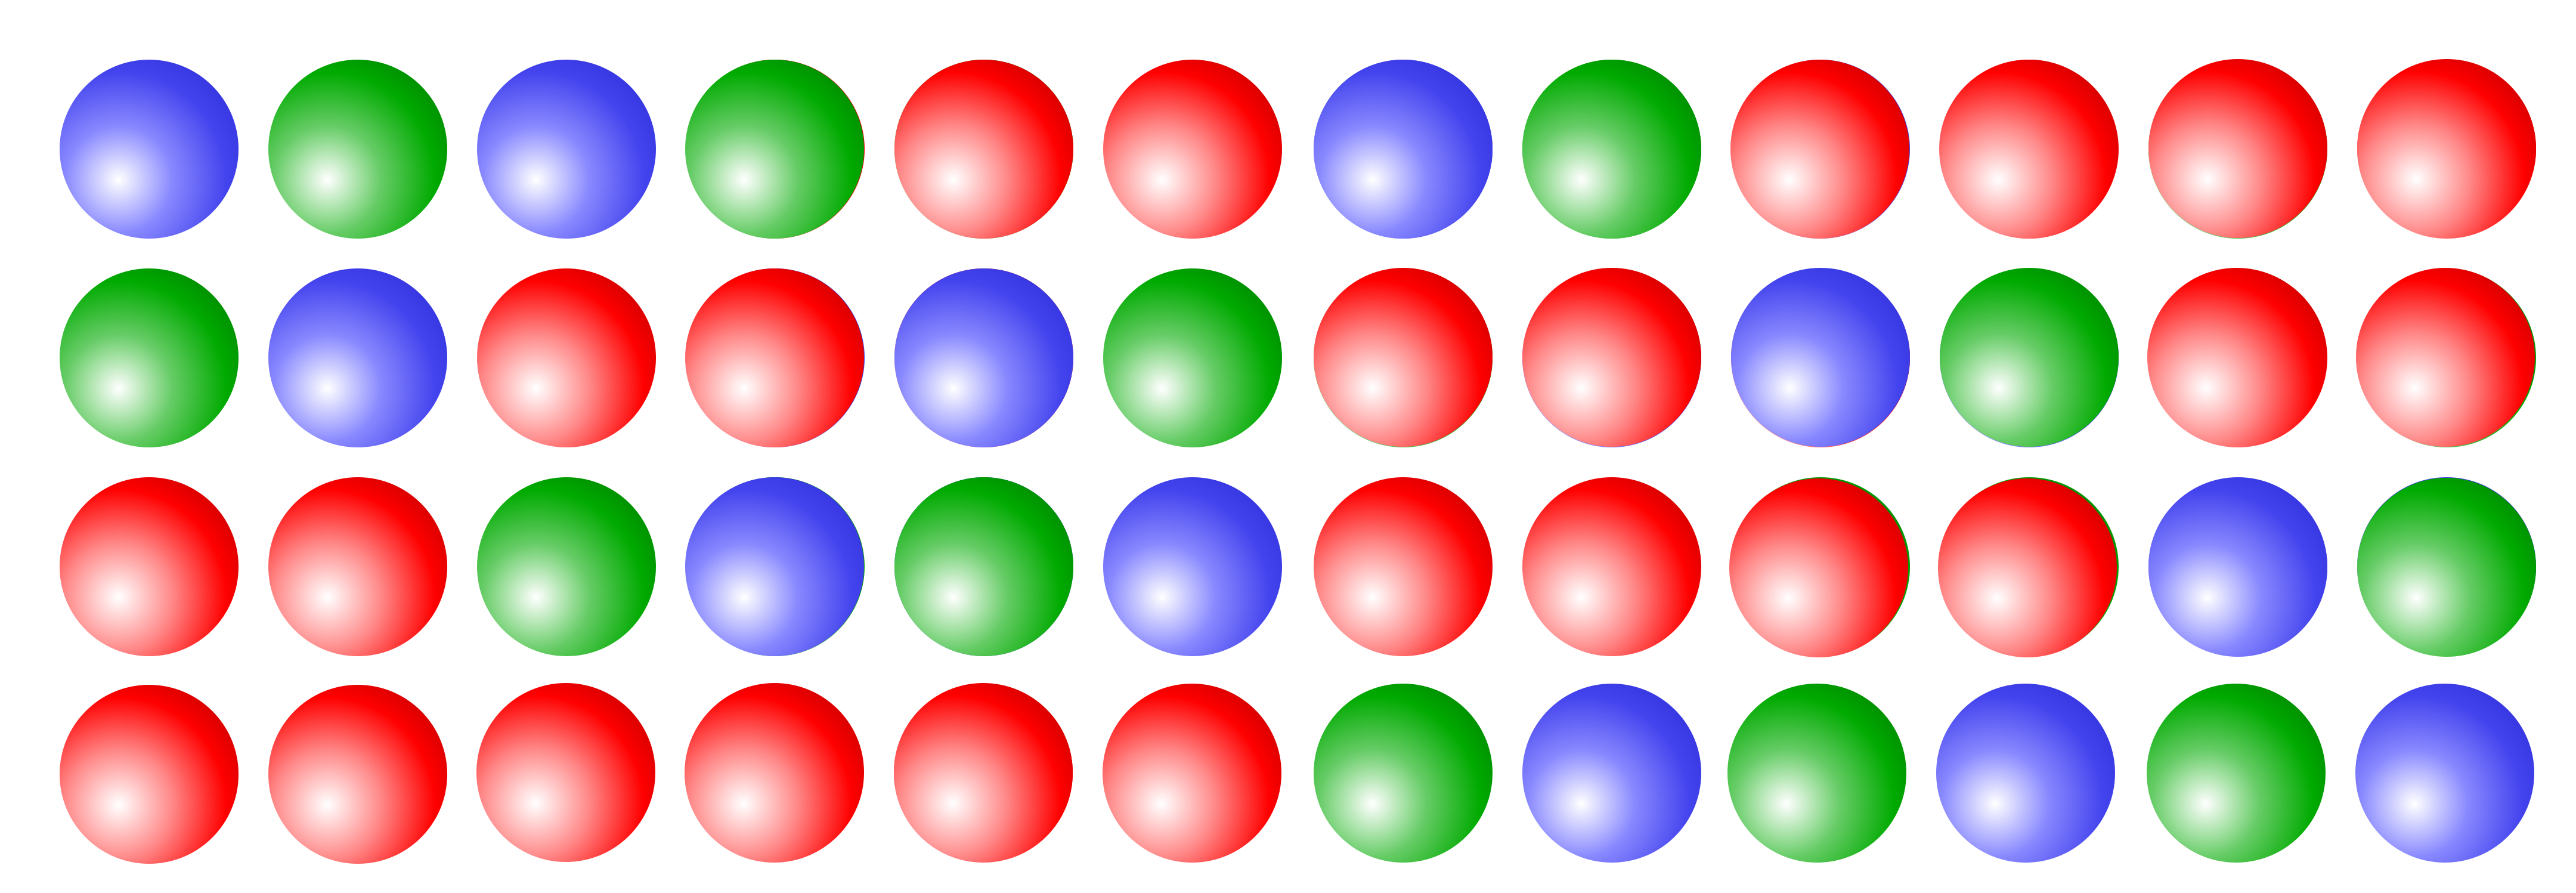
\includegraphics[width=0.8\textwidth]{permutations-2.png}\par}
\end{frame}
\begin{frame}{Пример. Перестановки с повторениями}
    \begin{exampleblock}{}
        Какова вероятность что из карточек с буквами \texttt{А,Н,А,Н,А,С} обезьяна сложит слово \texttt{АНАНАС}.
    \end{exampleblock}
    \begin{itemize}
        \item Так как число букв конечно и обезьяна не отдает предпочтений буквам, можно пользоваться формулой классической вероятности. 
        \item Количество исходов: Используются все буквы с заданными кратностями. Порядок важен. Это перестановки с повторениями.
        \item $n=P(3,2,1) = \frac{(3+2+1)!}{3!2!1!}=\frac{6!}{12}=60$
        \item Благоприятный исход один, поэтому $n(A)=1$.
        
        \item Итак,  \alert{$p(A)= \frac{1}{60}$}
    \end{itemize}    
\end{frame}
\begin{frame}{Размещения без повторений}
    Рассмотрим множество $A$, состоящее из $n$ элементов.
    \begin{block}{Определение}
        Кортежи длины $m$,  различающиеся либо составом элементов, либо порядком их расположения, либо и тем и другим, называются \alert{размещениями из $n$ по $m$}
     \end{block}
     \alert{Размещения без повторений}~--- все элементы в кортеже различны 
     $$
        \alert{A^n_m= n\cdot (n-1) \cdot \ldots \cdot (n-m+1) = \frac{n!}{(n-m)!}}
     $$
 
     \medskip
    %  \structure{Пример:}

    %  Рассмотрим размещения 4 цветов  по трем позициям: $A_4^3= \frac{4!}{(4-3)!}=24$

     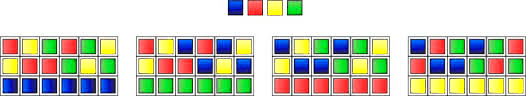
\includegraphics[width=\textwidth]{allocations.png}
\end{frame}

\begin{frame}{Размещения с повторениями}
    \begin{itemize}
         \item Размещения c повторениями~--- элементы в кортеже могут повторяться
         $$
            \alert{\tilde{A}^n_m= \underbrace{n \cdot n \cdot \ldots \cdot n}_m = n^m}
         $$
     \end{itemize}
\end{frame}
\begin{frame}{Пример}{}
    \begin{exampleblock}{}
        Код банковского сейфа состоит из 5 цифр. Найти вероятность того, что наудачу выбранный код подойдет.
    \end{exampleblock}
    \begin{itemize}
        \item Исходы --- введенные коды. их конечное число и вводятся наудачу.
        \item Число исходов порядок цифр важен и они могут повторяться, при этом используются не все. 
        \item Это размещения с повторениями из 10 по 5.
        \item \alert{$n=A_{10}^5=\frac{10!}{(10-5)!}=30240$}
        \item Событие $A$~--- код оказался верным. Благоприятный исход единственный. \alert{$n(A)=1$}.
        \item \alert{$p(A)=\frac{1}{30240}$}.
    \end{itemize}
\end{frame}

\begin{frame}{Сочетания без повторений}
    Рассмотрим множество $A$, состоящее из $n$ элементов.
    
    \begin{block}{Определение}
        $m$-элементные наборы множества $A$, отличающиеся только составом элементов, называются \alert{сочетаниями из $n$ по $m$}. 
    \end{block}
    \begin{itemize}
        \item Порядок элементов в сочетании не важен!
        \item Сочетания без повторений --- это $m$-элементные подмножества множества $A$.
    \end{itemize}
    $$
        \alert{C_n^k=\frac{n!}{k!\cdot (n-k)!}}
    $$
    {\centering 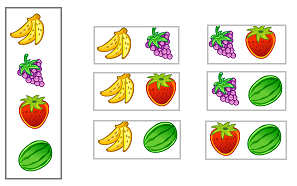
\includegraphics[width=0.43\textwidth]{combinations.png}\par}

\end{frame}

\begin{frame}{Сочетания без повторений. Пример}
    \begin{exampleblock}{}
        В группе 15 студентов, в том числе 8 отличников. Наугад выбраны 9 человек. Найти вероятность того, что среди отобранных ровно 5 отличников.       
    \end{exampleblock}
    \begin{itemize}
        \item Применим формулу классической вероятности.
        \item Опыт: выбор 9 человек из 15. Порядок выбора не важен, поэтому все исходы опыта --- сочетания.
        \item \alert{$n=C_{15}^9= \frac{15!}{9!6!}=\frac{15\cdot 14\cdot 13\cdot 12\cdot 11\cdot 10}{6\cdot 5 \cdot 4 \cdot 3\cdot 2}=5005$}
        \item Событие $A$~--- выбрано ровно 5 отличников и, следовательно, 4 не отличника. 
        \item \alert{$n(A)= C_{8}^5\cdot C_{15-8}^{9-5}=C_{8}^5\cdot C_{6}^{4}= \frac{8!}{5!3!}\cdot \frac{6!}{4!2!}=56\cdot 15=840$}
        \item Итак \alert{$p(a)=\frac{840}{5005}\approx 0.168$}
    \end{itemize}
\end{frame}

\begin{frame}{Сочетания c повторениями}
    Рассмотрим множество $A$, состоящее из $n$ элементов.
    
    \begin{block}{Определение}
        $m$-элементные неупорядоченные наборы множества $A$, допускающие повторения элементов и отличающиеся только составом элементов, называются \alert{сочетаниями из $n$ по $m$ c~повторениями}. 
    \end{block}
        $$
        \alert{\tilde{C}_n^k=\frac{(m+n-1)!}{m!\cdot (n-1)!}}
    $$
    {\centering 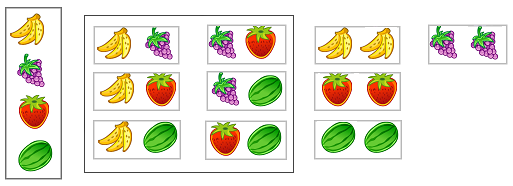
\includegraphics[width=0.75\textwidth]{combinations-2.png}\par}


\end{frame}
\begin{frame}{}
    \begin{exampleblock}{}
        По конвейеру, движутся конфеты четырёх наименований. Мы запускаем руки в этот поток и вытаскиваем двадцать штук. Какова вероятность, того, что среди выбранных есть конфета каждого наименования.
    \end{exampleblock}
\end{frame}
\begin{frame}{Комбинаторные соединения}{}
    \centering 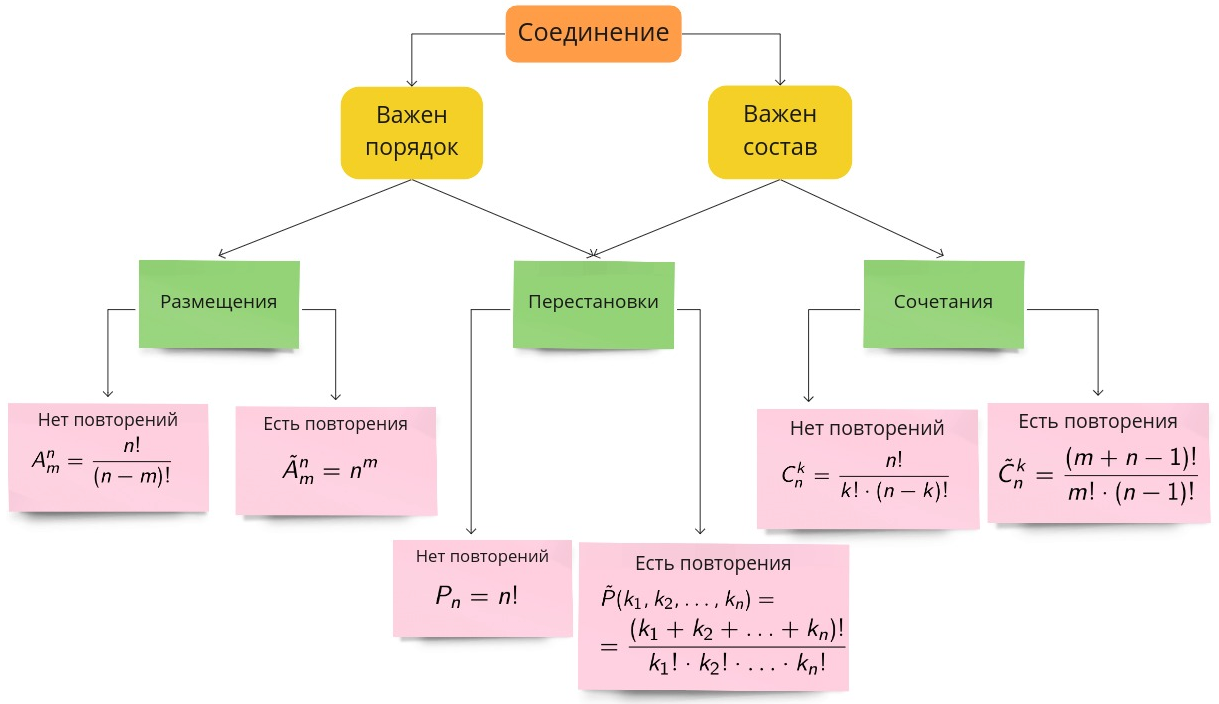
\includegraphics[width=1.05\textwidth]{diagram.png}\par
\end{frame}

\subsection{Геометрическая вероятность}
\begin{frame}{Идея геометрической вероятности}
    \begin{itemize}
        \item Допустим, пространство элементарных исходов опыта непрерывно.
        \item В этом случае формула классической вероятности неприменима.
        \item Определим формулу геометрической вероятности.
    \end{itemize}
    
    \bigskip
    Очень часто мы применяем формулу геометрической вероятности неявно:

    {\centering 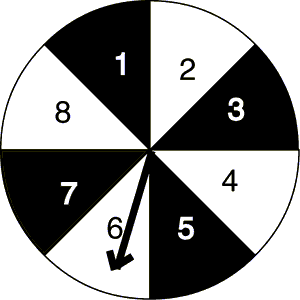
\includegraphics[width=3cm]{roulette.png} \par}

\end{frame}


\begin{frame}{Геометрическая вероятность}
        Пусть имеется некоторая область $\Omega$ и в ней содержится другая область $A$. 
    В область $\Omega$ наудачу бросается точка:
    \begin{itemize}
        \item брошенная точка может попасть в любую точку области;
        \item вероятность  ее попадания в область~$A$ не зависит от ее расположения и формы, а только от меры области $A$.
        \item Мера $||A||$~-- это длина, площадь, объем  исследуемой области $A$. 
    \end{itemize}

    \begin{block}{Геометрическая вероятность}
        Если исходы опыта и можно изобразить множеством точек некоторой фигуры, и вероятность события $A$ зависит только от меры $||A||$, то
        $$
            \alert{p(A)=\frac{||A||}{||\Omega||}}
        $$
    \end{block}
\end{frame}
\begin{frame}[allowframebreaks]{Геометрическая вероятность. Пример}{}
    \begin{exampleblock}{Задача}
        Два теплохода должны подойти к одному и тому же причалу. Время прихода обоих теплоходов независимо и равновозможно в течение суток. Определить вероятность того, что одному из них придется ожидать освобождения причала, если время стоянки первого теплохода шесть часов, а второго~--- восемь.       
    \end{exampleblock}
    \begin{itemize}
        \item Обозначим время прихода одного парохода как $х$, а второго как $y$.
        \item Ограничения: \alert{$0 \leqslant x \leqslant 24$, $0 \leqslant y \leqslant 24$}.
        \item Момент их прихода~--- точка квадрата со стороной 24.
        \framebreak
        \item Определим условия, когда первый пароход будет "мешать" второму. 
        Второй пароход грузится шесть часов, а в это время придет первый:
        $$
            \alert{x - y \leqslant 6,\qquad x\geqslant y}
        $$
        \item Теперь, второй пароход грузится восемь часов, а в это время придет первый:
        $$
            \alert{y - x \leqslant 8,\qquad y\geqslant x}
        $$
        \item Изобразим граничные условия на графике
        \framebreak

        {\centering \begin{tikzpicture}[x=1.7mm,y=1.7mm]
            \draw[->] (-1,0) -- (25,0) node[right]{$x$};
            \draw[->] (0,-1) -- (0,25) node[above]{$y$};

            \fill[blue!20] (0,0) rectangle (24,24);
            \fill[fill=vgured!20] (0,0) -- (6,0)-- (24,18)-- (24,24) -- (16,24) -- (0,8) --cycle;
            \draw 
                (6,0) node[below]{\small$6$}
                (0,8) node[left]{\small$8$}
                (24,0) node[below]{\small$24$}
                (0,24) node[left]{\small$24$}
                (0,0) node[below left]{\small$0$}
                ;
            \draw[thick,draw=vgured] 
                (6,0) -- node[sloped,below,vgured]{\small $x-y=6$} (24,18)
                (16,24) -- node[sloped,above,vgured]{\small $y-x=8$} (0,8);
            \draw[dashed,thick,draw=vgured] 
                (0,0) -- (24,24);

            \draw (12,12) node {$S_A$};
            \draw (20,4) node {$S_2$};
            \draw (4,20) node {$S_1$};
        \end{tikzpicture}
        \par}
        \item \alert{$||\Omega|| = S_\Omega = 24^2=576$}
        \item \alert{$||A|| = S_A=S_\Omega-S_1-S_2=24^2-\frac{16^2}{2}-\frac{18^2}{2}=286$}
        \item Итак, \alert{$p(A)=\dfrac{S_A}{S_\Omega}=\dfrac{286}{576}\approx 0.497$}.
    \end{itemize}
\end{frame}
\begin{frame}{Статистическая вероятность}
    Если не применима ни формула классической вероятности, ни формула геометрической вероятности используется формула статистической вероятности.
    $$
        \alert{p(A) \approx \frac{n(A)}{n}, \qquad n\text{~--- достаточно большое}}
    $$
    где $n(A)$~--- число появлений события $A$ в $n$ опытах.

    Важно понимать, что 
    \begin{itemize}
        \item она не является величиной постоянной;
        \item она зависит не только от числа проведённых испытаний, но и от условий их проведения.
    \end{itemize}
\end{frame}

\begin{frame}{Статистическая вероятность}
    При внешнем сходстве формул классической и статистической вероятностей они несут различную смысловую нагрузку, так 
    \begin{itemize}
        \item \structure{классическая вероятность}  указывает на вероятность появления события, которая является величиной постоянной для данного события, 
        \item \structure{статистическая}~--- характеризует всего лишь относительную частоту появления наблюдаемого события в проведённых испытаниях. 
    \end{itemize}
    
    {\centering 
\includegraphics[width=6cm]{Rosencrantz-and-Guildenstern-are-Dead.jpg}
    \par}
\end{frame}

\section{Теоремы о вероятностях}
\begin{frame}{Свойства вероятностей}{}
    Из определений канонической и геометрической вероятностей следует, что 
    \begin{itemize}
        \item Вероятность события $ 0 \leqslant p(A) \leqslant 1$.
        \item Вероятность достоверного события $p(\Omega)=1$.
        \item Вероятность невозможного события $p(\varnothing)=0$.
    \end{itemize}    
\end{frame}

\subsection{Независимые и зависимые события. Теоремы о произведении событий}
\begin{frame}{Независимые и зависимые события}
    \begin{itemize}
        \item Два события называются \alert{независимыми}, если вероятность одного события не зависит от того наступило другое или нет.
        \item Два события называются \alert{зависимыми}, если вероятность одного события зависит от того наступило другое или нет.
    \end{itemize}
    \structure{Пример:}
    \begin{itemize}
        \item В цехе работают две автоматические линии, выпускающие разную продукцию. При этом линии не конкурируют за ресурсы и не используют продукцию друг друга. В этом случае события остановки каждой из линий~--- независимы.
        \item В цехе работают две автоматические линии, выпускающие одну продукцию. Объем выпускаемой продукции в день фиксирован. В случае остановки линии вторая работает в ускоренном режиме. В этом случае события остановки каждой из линий~--- зависимы, так как повышается износ второй линии, а следовательно и вероятность ее остановки.
\end{itemize}
\end{frame}
\begin{frame}{Условная вероятность}
    \begin{block}{}
        \alert{Условная вероятность}~\alert{$p(A/B)$}~--- вероятность события $A$, вычисленная при условии, что имело место другое событие $B$. 
    \end{block}
    
    $$
        \alert{p(A/B)={}} \frac{n(A\cap B)}{n(B)} 
        =\frac{\frac{n(A\cap B)}{n}}{\frac{n(B)}{n}}
        \alert{{}=\frac{p(AB)}{p(B)}
        }
    $$
    {\centering 
     \begin{tikzpicture}[x=10mm,y=6mm]
        \draw (-2.5,-2.6) rectangle (4.5,2.6);
        \filldraw[draw=black,thick, fill=red!50, fill opacity=0.7] 
            (0,0) circle[radius=2];
    
        \filldraw[draw=black,thick, fill = yellow!50, fill opacity=0.5] 
            (2,0) circle[radius=2];
        \draw 
            (-2,2) node {$\Omega$}
            (-1,0) node {$A$}
            (3,0) node {$B$}
            (1,0) node {$A \cap B$}
            ;
    \end{tikzpicture}        
    \par}

\end{frame}
\begin{frame}{Произведение событий}{}
    
    \begin{theorem}[о произведении событий]
        $$
        p(AB)=p(A/B) \cdot p(B) =  p(B/A) \cdot p(A)
        $$
    \end{theorem}

    \bigskip
    События независимы тогда и только тогда, когда
    $$
        P(A) = P(A/B);\qquad   P(B) = P(B/A).
    $$
    \begin{theorem}[о произведении независимых событий]
        $$
        p(AB)=p(A) \cdot p(B) 
        $$
    \end{theorem}
\end{frame}
\begin{frame}{Пример применения произведения событий}
    
\end{frame}
\subsection{Несовместные и совместные события. Теоремы о сумме событий}

\begin{frame}{Несовместные и совместные события}{}
\begin{block}{Определение}
    События  $A$ и~$B$ называются
    \begin{itemize}
        \item  \alert{несовместными}, если появление одного из них исключает появление других;
        \item \alert{совместными}, если наступление одного из них не исключает наступления другого.
    \end{itemize}
\end{block}

\structure{Пример:}
При броске игральной кости, рассмотрим события:
\begin{itemize}
    \item $A_1$~--- выпадение нечетного числа очков.
    \item $A_2$~--- выпадение 6.
    \item $A_3$~--  выпадение  2 или 4.
    \item $B$~---   выпадение числа очков меньше 3.
\end{itemize}
{\centering\color{vgured}\begin{tabular}{cc}
    Не совместные & Совместные \\
    $(A_1, A_2, A_ 3)$ & $(A_1, B)$\\
    $(A_2, B)$         & $(A_3, B)$\\
\end{tabular}\par}
\end{frame}

\begin{frame}{Сумма событий}{}
  
    
    \alert{Суммой $A+B$} событий $A$ и $B$ называется событие, состоящее в наступлении хотя бы одного из этих событий.
    
    {\centering 
     \begin{tikzpicture}[x=10mm,y=6mm]
        \draw (-2.5,-2.6) rectangle (4.5,3);
        \fill[fill=vgured!50] 
            (0,0) circle[radius=2];
        \fill[fill=vgured!50] 
            (2,0) circle[radius=2];
        \draw 
            (0,0) circle[radius=2]
            (2,0) circle[radius=2];            
        \draw 
            (-2,2) node {$\Omega$}
            (-1,0) node {$A$}
            (3,0) node {$B$}
            (1,2.5) node {$A + B$}
            ;
    \end{tikzpicture}        
    \par}    
    \begin{block}{Теоремы о сумме событий}
        \begin{itemize}
            \item Сумма зависимых событий \alert{$p(A+B)=p(A)+p(B)-p(AB)$}
            \item Сумма независимых событий \alert{$p(A+B)=p(A)+p(B)$}
            \item Противоположные события \alert{$p(\bar{A})=1-p(A)$}
        \end{itemize}
    \end{block}
\end{frame}

    \begin{frame}{Пример вероятности суммы событий}{}
        \begin{exampleblock}{Задача}
            В торговом центре два одинаковых автомата продают кофе. 
            Вероятность того, что к концу дня  в автомате закончится кофе, равна 0,3. 
            Вероятность того, что кофе закончится в обоих автоматах, равна 0,12. 
            Найти вероятность того, что к концу дня кофе закончится хотя бы в одном из автоматов.
        \end{exampleblock}
        \begin{itemize}
            \item $A$~--- «кофе закончится в первом автомате» \hfill \alert{$p(A)=0.3$};
            \item $B$~--- «кофе закончится во втором автомате» \hfill \alert{$p(B)=0.3$};
            \item события являются совместными, так как \hfill \alert{$p(AB)=0.12 \neq 0$}.
            \item \alert{$p(A+B)= p(A)+p(B)-p(AB) = 0.3+0.3-0.12 = 0.48$}.
        \end{itemize}
    \end{frame}

\begin{frame}{Полная группа событий}{}
    \begin{block}{}
        События $H_1, H_2,\ldots, H_n$ образуют \alert{полную группу событий}, если 
        \begin{enumerate}
            \item события \alert{$H_1, H_2,\ldots, H_n$} попарно \underline{несовместны};
            \item \alert{$H_1+H_2+\ldots+H_n = 1$}
        \end{enumerate}
    \end{block}

    \bigskip
    \begin{itemize}
        \item События образуют полную группу, если в результате опыта происходит ровно одно из них.
        \item Все исходы опыта образуют полную группу событий.
        \item Событие $A$ и противоположное к нему событие $\bar{A}$ образуют полную группу событий.
    \end{itemize}
\end{frame}

\subsection{Формула полной вероятности}

\begin{frame}{Полная вероятность}
    Следствием теорем о вероятностях   является формула полной вероятности:
    \begin{theorem}{}
        Если 
        \begin{itemize}
            \item $H_1,H_2,\ldots, H_n$~--- полная группа событий;
            \item известны условные вероятности $p(A/H_i)$ для всех $i\in \{1,2,\ldots,n\}$,
        \end{itemize}
        то
        $$
           \alert{p(A) = \sum_{i=1}^n p(H_i)p(A/H_i) =p(H_1)p(A/H_1)+ \ldots+p(H_n)p(A/H_n)}
        $$
    \end{theorem}
\end{frame}

% \begin{frame}{ФОрмула Байеса}
%     Следствием теорем о вероятностях   является формула полной вероятности:
%     \begin{theorem}{}
%         Если 
%         \begin{itemize}
%             \item $H_1,H_2,\ldots, H_n$~--- полная группа событий;
%             \item известны условные вероятности $p(A/H_i)$ для всех $i\in \{1,2,\ldots,n\}$,
%         \end{itemize}
%         то
%         $$
%             p(A) = \sum_{i=1}^n p(H_i)p(A/H_i) =p(H_1)p(A/H_1)+ \ldots+p(H_n)p(A/H_n)
%         $$
%     \end{theorem}
% \end{frame}
% \section{Формула Байеса}
\end{document}
